\part{Methods and implementation}
\label{pa:methods}
\chapter{Cytoscape}
\section{Intro}
The \textit{clusterMaker2} documentation for implementing new parts that is not
directly connected with clustering algorithms is non-existing. This part
explains the details about how it was done.

Cytoscape has a cookbook\cite{cytoscape-cookbook} listing a combination of best
practices and tips on how to start developing an app, add menues, panels,
algorithms, color schemes etc.. Instead of following all of these examples, we
have read through the existing code in clusterMaker2\cite{cm2-github} and tried
to structure the code of the contributions in Ranklust to match the structure
already implementet in clusterMaker2. Meaning that for each algorithm
implemented, they will all have a corresponding \textit{Factory} class and a
\textit{Context class}. For the panel that was implemented, it has a pure panel
class with Java Swing\cite{java-swing} settings, a panel task class, create
panel task class and destroy panel task class.

\section{Workflow and usage}
\subsection{Installation}
At the moment, clusterMaker2 does not officially contain Ranklust. So in order
to use Ranklust, the user are required to compile the Java source code or
download the updated JAR-file\cite{jar}(URL: \url{
https://github.com/henninglh/ranklust-app/ranklust-1.0.0.jar}). To build this
whole project I have used Maven as a build tool\cite{maven}. To compile the
project into an executable JAR-file Cytoscape can use, \gls{maven} has to be
instructed to skip all tests, because the current tests has compilation errors.

\textbf{Skipping tests with maven:}
\begin{Verbatim}[fontsize=\scriptsize]
mvn clean install -Dmaven.test.skip
\end{Verbatim}

The JAR-file that is being produced after the line over is executed in
a terminal or through the build tool of an \gls{ide}. This file has to be put in
the configuration folder of Cytoscape. The location of the configuration folder
can vary across operative systems and Cytoscape versions, but the Cytoscape
version 3.4.0 follows this path:
\begin{Verbatim}[fontsize=\scriptsize]
<user home folder>/CytoscapeConfiguration/3/apps/installed/<put the jar here>
\end{Verbatim}

After this step is done, the user can start up Cytoscape and should be able to
Ranklust.

\subsection{Researcher workflow}
The way researchers can use Ranklust is pretty simple. Step 1 and 2 will only be
required the first time the researcher want to use this app to solve his/her
problem. The rest has to be done every time, unless a previous session of
Cytoscape is loaded with more developed results.

\begin{enumerate}
    \item Install Cytoscape
    \item Install clusterMaker2 plugin through Cytoscape App manager
    \item Upload the network to be clustered and ranked into Cytoscape
    \item Use clusterMaker2 to cluster the network
    \item Use the Ranklust-part of clusterMaker2 to rank the clusters
        \begin{enumerate}
            \item Decide what to score the clusters on
        \end{enumerate}
    \item Use the Ranklust-part of clusterMaker2 to visualize the rankings
\end{enumerate}

Step 6 should show the researchers the ranking of clusters based on what
attributes they wanted to include in step 5a. This ranking represents cluster
biomarkers. The score of the clusters and the order they are ranked in will
decide the state of the patient. State of the patient can be many different
things and what the rankings will mean to the researcher is not yet final. It
will be a new indicator, a biomarker, and information about what it means has to
be gathered empirically through clinical research.

\section{Maven and the POM file}
The POM-file has to be updated because libraries connected to the pdf exporting
functionality is outdated. Updating the libraries, imports and the usage of
these libraries in the source code is enough to make the whole project compile.
Also, in order to get the third-party libraries to JUNG\cite{jung} into the
project, the three packages that is being used has to be added to the POM file
and the classes they contain has to be exposed in the OSGi
module\cite{osgi-felix}. Exposing the JUNG classes inside the clusterMaker2 OSGi
bundle could have been avoided if JUNG had OSGi modules in maven repositories,
but there is only 2 out of 3 OSGi ready modules that was needed in this project.
These were the changes needed:

Changed which packages was exported through the OSGi module.

\begin{lstlisting}[language=XML, caption={POM-file OSGi changes}]
<Export-Package>!${bundle.namespace}.*,*;-split-package:=merge-first</Export-Package>
\end{lstlisting}

Added these dependencies

\begin{lstlisting}[language=XML, caption={POM-file JUNG changes}]
<dependency>
    <groupId>net.sf.jung</groupId>
    <artifactId>jung-graph-impl</artifactId>
    <version>2.1</version>
</dependency>
<dependency>
    <groupId>net.sf.jung</groupId>
    <artifactId>jung-algorithms</artifactId>
    <version>2.1</version>
</dependency>
<dependency>
    <groupId>net.sf.jung</groupId>
    <artifactId>jung-api</artifactId>
    <version>2.1</version>
</dependency>
\end{lstlisting}

As seen here, the 3 modules needed is jung-api, jung-graph-impl and
jung-algorithms. Only the first 2 was OSGi ready. An alternative could have been
to create a OSGi ready module of the jung-algorithms module, but taking on the
responsibility for having a module updated at all times is too much for a single
person. However, it could become the clusterMaker2's developers responsbility to
create and update all 3 modules. The last alternative is to find other graph
ranking algorithm libraries like Apache Spark\cite{spark}, thas is OSGi ready.
The reason for not choosing Apache Spark is that it was not discovered until all
of the Java implementation was finished, making it a future goal to reach, at
best.

\section{App registration and java class connections}
First step of registration is to register a \textit{service listener} to the
already existing clusterMaker2 \textit{CyActivator}. Here I describe the name
of java methods in the \textit{clusterManager} class with strings. These two
methods for adding and removing ranking algorithms registers and unregisters the
algorithms to the \textit{App} menu in Cytoscape, making them accessible for the
user through the GUI. Registering a new service listener is a way of keeping the
Ranklust part out of clusterMaker2. Also, creating a standalone plugin at
a later stage will be easier if Ranklust is properly compartmentalized.

The \textit{RankFactory} class is a java public interface used for each of the
ranking cluster algorithms, \gls{hits}, \gls{pr}, \gls{prwp}, \gls{maa} and
\gls{mam}. A class applying the task factory design pattern is meant to deliver
an object of the class it is related to\cite{factory-design}, and it can return
different types of a class that has the same java
superclass\cite{java-superclass}. In this case, each class implementing the
\textit{RankFactory} will only have a single class to return. The RankFactory
class also creates a \textit{Context} class, which binds information the user
can input to the GUI to variables, allowing the algorithm to gain access to
parameter information about the algorithms before they run.

\section{Algorithms for ranking clusters}
Each ranking algorithm has atleast three classes, like the clustering
algorithms. A context class responsible for handling GUI elements visible to the
user and to convey the parameters and attributes the user sets. A TaskFactory
class responsible for registering the algorithm with the CyActivator class and
to encapsule the class executing the ranking algorithm in a TaskIterator class.
The TaskIterator class is required for every task that is to be executed in
Ranklust. This is to have control over the sequence that tasks was added to in
the Cytoscape environment. The third required class is the algorithm class
itself. It has to contain certain methods in order to compile, but the most
important one is the run() method, which is the method that is called in order
to initialize the execution of this class, and as a result of that, the
algorithm itself.

For every ranking algorithm in Ranklust there is some steps that every ranking
algorithm has in common:
\begin{enumerate}
    \item Initialize progress bars displayed to the user
    \item Retrieve the clusters through the ClusterUtils.fetchClusters() method
    \item Initialize other variables needed
    \item Retrieve node and edge attributes from the Context class
    \item Insert nodes and edges into a graph (only for PR, PRWP and HITS)
    \item Execute graph algorithm in JUNG (only for PR, PRWP and HITS)
    \item Collect and summarize values, create average cluster values and
        normalize the values
\end{enumerate}

\section{The results panel from ranking clusters}
The code for the \textit{RankingPanel} is a copy from the existing
\textit{ResultsPanel} in clusterMaker2. The results panel has some extra
information that is removed in the ranking panel. The ranking panel only
displays which clustering and ranking algorithm that was used and the network it
is used on, together with the score of each cluster sorted descendingly, having
the highest ranked cluster at the top. The ranking panel will display in the
same place as the results panel, to the right of the network view.

The panel supports multiple selection of clusters through the \textit{Control}
key on the keyboard, much like its existing behaviour on Windows when selecting
multiple directories or files in the \textit{File Explorer}. Selecting the
clusters in the panel will also select them in the network view, enabling the
user to use other Cytoscape utilities on the nodes/clusters selected, for
example create a new network based on only the selected nodes. The color of the
selected nodes will also change in the network view, when the user selects a
cluster in the ranking panel, providing visual feedback to the user, in order to
make it easier for the user to see where the selected nodes/clusters resides in
the network.

When tasking clusterMaker2 with showing the ranking panel, the color of the
nodes will also change. This is to visualize the rank of each cluster in the
network view to the user. Coloring the highest scoring clusters with red or
green and the lowest scoring with the opposite was the first and easiest
solution. There was made a choice to color the whole cluster according to the
rank it received, instead of individually color nodes according the their
contribution to the clusters rank. The user might be interested in choosing what
suits them best when it comes to this, so it might be implemented a menu for the
ranking panel in the future to best meet the users needs.

Taking color blind people into consideration red and green is not the
best combination. Colors resembling red and green in the form of hot-to-cold
colors that all types of colorblind people can view was therefore a criteria to
be met. A style satisfying these criteria will follow, having the hex value of
te color\cite{color-blindness3}, followed by the RGB value that was calculated
using a site that converts from hex to RGB values\cite{color-blindness2}.
\textit{\#ADD rgb\(170,221,221\)} for a blueish and cold color representing low
score. \textit{\#FEC rgb\(255,248,204\)} represents off-brown color that is a
step warmer than the blueish. The warmest color representing the highest scored
clusters is \textit{\#F99 rgb\(255,153,153\)}. The drawback with this color
combination is with people that has color blindness to the degree where they see
only greyscales. The colors low to high will go from grey to light grey to dark
gray, which does not seem logical. The color style might change if users
experience trouble having these colors representing the cluster ranks. 

\section{Current state of development}
The pull request\cite{git-pull-request} made from the Ranklust
contribution of this thesis has been accepted\cite{ranklust-accepted}, adding
3750 lines of code and deleting 1051. The changes was distributed across 50
files. The type of files edited ranges from the Maven POM-settings file and
.gitignore to plain Java source code files. Further changes will be made, as the
work on the Ranklust contribution will not end when this thesis is delivered.
One of the most recent changes to the contribution is that the
\textit{PageRankWithPriors} algorithm used to analyze the networks in this
thesis assumes undirected edges because of the
\textit{UndirectedSparseMultigraph} graph used. For normal use, directed edges
is believed to be the most sought after choice. Therefore, the pull request was
hardcoded with directed edges. Choosing between directed and undirected edges
should in the end be up to the users of clusterMaker2 and is on the TODO-list of
futures to implement.

\section{Known bugs}
\subsection{Menu bugs}
\paragraph{Unintentional execution of clustering algorithm}
\begin{enumerate}
    \item Open the clusterMaker2 clustering algorithm menu
    \item Select a clustering algorithm
    \item Exit the menu for the algorithm without running it
    \item Repeat step 1-2 for the same algorithm and it results in running the
        previous algorithm that was exited without displaying the parameter
        prompt
\end{enumerate}
This was the behaviour before Ranklust was added to clusterMaker2,
so it might be clusterMaker2 or it might be Cytoscape itself. Most likely, the
way clusterMaker2 algorithms is started through its \textit{TaskFactory}'s needs
to be changed, but this is just a hunch and not based on any analysis.

\subsection{Ranking panel bugs}
It is a known bug with the style for node coloring that the ranking panel
causes. The colors in the nodes might flicker when several ranking algorithms
has been run and the colors of each node has changed several times. This is
probably related to the previous color style for the nodes and it will be fixed
in the future.

\section{Clustering}
PPI networks already have a great deal of edges, and can be seen as clusters
that I should not alter. On the other hand, using clustering algorithms to make
clusters out of PPI-networks gives us the more control over the clusters and has
the potential to identify protein complexes\cite{ap-vs-mcl}. How big they should
be, how many of them I want, should I cluster on a certain attribute, or even
several? I have chosen to go with the \textit{Markov Cluster}(MCL)\cite{mcl}
clustering algorithm in \textit{clusterMaker2}, without any limitations to the
amount of clusters or weighting of the nodes. I prototyped Ranklust with
\textit{Affinity Propagation}(AP)\cite{affinity-propagation} because of its ease
of use and low execution time, but through a comparison between MCL and AP, it
was concluded with MCL having better performance in many aspects when it came to
cluster unweighted PPI networks\cite{ap-vs-mcl} with binary interactions. These
aspects being noise tolerance and more robust behaviour, which will contribute
greatly to cluster the iRefWeb network.

\section{Ranking clusters}
I have used five algorithms to rank the clusters, Multiple Attribute Additive
Method (\gls{maa}), Multiple Attribute Multiplication Method (\gls{mam}),
PageRank (\gls{pr}), PageRank with Priors (\gls{prwp} and Hyperlink-Induced
Topic Search (\gls{hits}). The first two are simple algorithms that through
addition or multiplication calculates a cluster's average score. The three
others utilize network ranking algorithms from the Java JUNG\cite{jung} library.

Every algorithm implemented in Ranklust for ranking clusters except \gls{hits}
takes node and/or edge scores as input for calculating the scores for each
cluster.

\subsection{Multiple Attribute Additive Method (MAA)}
Multiple attribute additive method is the first algorithm implemented.  The user
has the option of choosing an unlimited amount of attributes from nodes and
edges.

It goes through all of the nodes in each cluster and sums up the number-
attributes the user chose. Each cluster is then ranked based on the average sum
in each cluster and ranked descending, with the highest ranking cluster as the
most likely prostate cancer biomarker cluster.

There is a question as to how to rank the edges in the cluster. We chose to rank
each edge as it is listed to the user in Cytoscape. So if it is listed only once
time in the edge table, it will only be scored additively once. This decision
was based on simplicity. To not represent the edge as something the user did not
define it as, or is unable to understand. Some clustering algorithms might
assign the same node or edge to several clusters, though this is not the case
with the algorithms I use in this thesis. Support for this is only implemented
by \gls{maa} and \gls{mam}, as they were implemented before a final decision on
which clustering algorithms should be used. If \gls{maa}/\gls{mam} discovers
this special case of several scores for a single node or edge, it will assign it
the highest value.  The reason for leaving this feature in Ranklust is to have
an example on how it can be done, should it be a problem in the future.

\subsection{Multiple Attribute Multiplication Method (MAM)} Multiple attribute
multiplication method is to some degree redundant, considering what exists from
before in Ranklust. The only difference from \gls{maa} is the scale the scores
will be in. \gls{maa} adds the scores from each node and edge in the cluster
through addition, \gls{mam} does it with multiplication.

A problem that occurs with multiplication is calculating scores for clusters
that contain nodes with a score between 0 and 1, since the score would decrease
to such a degree that it would be difficult to work with when normalizing the
scores. The solution I have chosen for this problem is to make a new score from
the score that is to be added to the cluster average, and add 1.0 to it. This
way, when the existing average score in the cluster is multiplied with the new
score, it will always increase, unless the old value was 0.0, or both the old
and the new value was 1.0. In the case of values above 1, they will also be
given an increase by 1.0 in order to keep it consistent if the scores vary
between 0 to \textit{n}. Normalizing every value before running the algorithm
contributes to keep all of the values between 0 and 1, and in that way prevent
scaling problems when adding 1.0 to a score over 1.0. The whole reason to add
1.0 was to counteract the problem with the score decreasing when it should be
increasing.

\subsection{PageRank (PR) and PageRank with Priors (PRWP)} 
A Random Walks\cite{random-walks2} algorithm which used priors, called
seed-weighted random walks ranking \cite{sw-rwr}, proved to be effective at
prioritizing biomarker candidates. PageRank (\gls{pr}) is an algorithm based on
the Random Walks principle, and it is contained inside the Java library
\textit{JUNG}\cite{jung}. PageRank was previously used by Google to rank
webpages \cite{pagerank}. PageRank with Priors (\gls{prwp})\cite{pr-bio} is a
modified version of \gls{pr}, where nodes and edges can be assigned a score
prior to the \gls{pr}'s traversal of the network. \gls{pr} can have values
assigned to the edges, but it does not require any scores in order to rank
clusters, which \gls{prwp} does. PageRank with Priors is abbreviated \gls{prwp}
because of the Java classname it has in the Java JUNG library
- \textit{PageRankWithPriors}.

The difference between \gls{maa} and \gls{mam} compared to \gls{pr} and
\gls{prwp} is how the network is scored. \gls{maa} and \gls{mam} calculates the
score for each cluster by summing up the attributes in edges and nodes according
to the cluster attribute. \gls{prwp} scores the current network regardless of
the clustering attribute. 

MCL gives the option of creating a clustered network, which opens up the
possibility of working with two types of the same network, non-clustered and
clustered. They both have the clustering attribute in the network, edge and node
table, so that the ranking algorithms are able to score the clusters. \gls{prwp}
scores the currently selected network in Cytoscape, resulting in the option of
scoring the non-clustered network or clustered network. The last option gives
the clustering algorithm a bigger impact on the score, because the clustered
network has perturbated edges between nodes that is not in the same cluster. MCL
in Cytoscape can show the "inter-cluster" connecting edges, which is the egdes
that was perturbed during clustering. This last option is a combination of the
two others. It will be visually close to the clustered network, but algorithms
that run on the network with inter-cluster edges will have the same result as
the network only containing the cluster attribute.

Implementation wise, there is also a difference in how the scores are stored in
the network after the algorithm is finished executing. All the scores are stored
in the nodes. To give information to the user about the scores the edges
received, each edge will display the total score for the cluster it is a member
of, just like the nodes. Only \gls{prwp} and \gls{pr} will also display the
single node score.

\subsection{Hyperlink-Induced Topic Search (HITS)}
Hyperlink-Induced Topic Search, \gls{hits}, an algorithm that is similar to
PageRank, was developed around the same time \cite{hits}\cite{hits-origin} and
is also contained within the Java JUNG library. \gls{hits} will not be used to
calculate cluster scores and ranks, due to the fact that it does not require any
form of weighting in nodes or edges. Though, it can be used in combination with
other ranking algorithms through the use of \gls{mam} or \gls{maa}. 

An example of this could be running \gls{prwp} with a score attribute, then
\gls{hits} on the same network. The next step would be to combine the two scores
from \gls{prwp} and \gls{hits} with \gls{maa}. Though, the idea of achieving
novel information on network biomarkers for prostate cancer through this
workflow is pure speculation, and we have chosen to use each ranking algorithm
separately, in order to limit the amount of datasets to analyze.

\subsection{PR, PRWP and HITS}
Because \gls{pr}, \gls{prwp} and \gls{hits} rely on an alpha variable
controlling the probability of a reset in the traversal of the network. This
"traversal reset" is automatically triggered if the algorithm hits a node with
no outgoing edges. As the clustering algorithms might change the edges in the
network, the outcome of performing ranking on a cluster-created network, versus
a network with only a cluster attribute to identify the clusters, can
potentially be vastly different. I have decided to not use the cluster-created
network, and instead use the network with cluster attributes. The perturbation
of edges in the network and separation of nodes into a more disconnected graph
might hide interactions in the network that can provide useful information to
\gls{prwp}. On the other hand, it might produce more noice in the network and
skew the ranking of the clusters through interactions that are false positives,
regarding protein complex interactions. 

The alpha value parameter will be set to 0.3. This specific alpha value has been
proven to be effective in both identifying and prioritizing candidate genes in
diseases\cite{disease-prwp}. Another parameter for \gls{pr}, \gls{prwp} and
\gls{hits} is the iteration parameter. For each iteration of these algorithms,
they assign a value to each node. Performing multiple iterations contribute to
stabilize these values. In the previously mentioned report from Google
\cite{pr-parameters}, a \textit{n x n} matrix where \textit{n} was about 25
billion, required about 50 - 100 iterations in order to stabilize the node
values. Iterations needed to stabilize increase with the size of the network,
therefore the iteration value to start with will be 30. It is a little less that
what Google has specified, but in contrast, the iRefWeb network is 9500 nodes
big, with approximately 43,000 edges, which is a considerably smaller network
than "the internet", which Google tried to rank.

\chapter{Programming specifics}
\section{OSGi and design patterns}
Developing OSGi software promotes modularization \cite{modularization} of the
code and increase the probability of the app being launched as an official
Cytoscape app; in addition to provide other developers with the possibility of
reusing my modules in their own apps. Also, it seems like Java 9 is aimed at
making it easier to modularize apps along the lines of the OSGi
standard\cite{jigsaw}, so it might be easier to refactor an application in the
future from Java 8 to Java 9 when the architecture already is in place. There
exists several design patterns that could prove to be useful in the development
of Ranklust. Another strategy to follow may not be a direct design pattern
\cite{designpattern}, but more of a collection of them, and it is the clean
code principles by Robert C. Martin \cite{cleancode}. Going against the coding
principles promoted by the Cytoscape app community and exclude the use of OSGi
modules will not be done, but third party Java libraries that is not OSGi-ready
will be used, namely the JUNG library\cite{jung}.

\section{Tables vs pure OO}
One thing in particular that deserves to be mentioned is the way networks are
handled. The \textit{CyNode} objects, which represents a single node, does not
contain much. This is because all of the information is saved in the form of
plain cells in a spreadsheet. This may at first seem like a way to make it easy
to show information to the user, but it is also a way of working more efficient
with network graph data. Creating objects with attributes for each node in a
huge network will increase the amount of overhead. Working with all of the
information in the way of a spreadsheet with rows and columns results in a
decrease in overhead. A new node is a new row in the node table, so in relation
to building the network structure, it is not a complex abstraction.  The
difference comes in when the nodes have several attributes. 

In a table or spreadsheet, attributes can be represented as a single column and
be created once for the whole network, instead of once for each node object
created. This assumes that getting the objects out of the table is possible by
either indexing on a number for arrays, or a unique key for map structures.
The result is both a lookup, insertion and deletion time of O(1). These times is
as low as the Big-O notation goes in terms of speed related to the size of
a collection inside a data structure. So both the creation of objects goes
down, and the retrieval of attribute information is as low as it is possible to
get, when I choose to represent the time by Big-O notation. The only drawback
with this implementation is that there is no current type of wrapper around the
row and column system. So the retrieval of information is not done the most
intuitive way. This is the way Cytoscape works as a whole, so changing the
way this works can either be done through changing the Cytoscape source code, or
implementing a wrapper as a standalone function inside clusterMaker2 or as
a standalone plugin. In Ranklust, an extension to the existing
\textit{NodeCluster} class was used to keep scoring information about nodes in
clusters.

\section{Changes in existing classes}
\subsection{NodeCluster}
\begin{Verbatim}[fontsize=\scriptsize]
/**
 * In it's simplist form, a Cluster is a group of nodes that represents the
 * nodes that are grouped together as the result of a clustering algorithm
 * of some sort.  A more complicated form of a cluster could include clusters
 * as part of the list, which complicates this class a little....
 */
\end{Verbatim}

This comment is in the NodeCluster class. In the Ranklust implementation,
several attributes and methods has been added to this class. Saving the
temporary state of the scores to the clusters could have been done in the node
and edge-tables in Cytoscape, but it was faster both implementation- and
performance-wise to extend the NodeCluster class. Also, a criteria for extending
this class was that the existing API of this class should not change, in order
to avoid unneccessary changes for other classes in clusterMaker2, that is not
a part of Ranklust. 

Additions to NodeCluster contains variables representing cluster \textit{score},
\textit{rank} and a \textit{HashMap} from a cluster-node's SUID to its score.
The map and rank variables is part of a previous implementation and can be
removed. Adding node scores to the cluster and normalizing it afterwards.

\textbf{Common responsibilities introduced in Ranklust}
\begin{itemize}
    \item Adding node scores to the cluster (ranking algorithm related)
    \item Normalizing cluster scores for a list of clusters (static method)
    \item Calculating min/max/avg scores for a list of clusters (static method)
    \item Ranking a list of clusters by their score and set their rank
        accordingly (ranking panel related)
\end{itemize}

\subsection{GraphicsExportPanel}
Minor changes were done to GraphicsExportPanel when a new class for handling PDF
documents was introduced. This was the result from the need to change the maven
dependency to use the "com.itext"\cite{itext} repository location instead of
a location from "com.lowagie" because the library was relocated
\cite{lowagie-to-itext}.

\section{New classes}
\subsection{ClusterUtils}
\textit{ClusterUtils} is a new class implemented in the Ranklust contribution.
It is used by every cluster ranking algorithm implemented in Ranklust. To some
degree it has a common responsibility with the \textit{ModelUtils} class from
clusterMaker2. The difference being that ClusterUtils is focused on inserting
scores in tables related to cluster ranks. It also normalizes scores not
directly related to a NodeCluster, but rather a group of \textit{CyNodes}, that
has mapped their SUID in Cytoscape to a score received from a ranking algorithm.

\textbf{Common responsibilities introduced in Ranklust}

\begin{itemize}
    \item Getting cluster attribute based on CyNetwork
    \item Getting ranking attribute based on CyNetwork
    \item Ranking clusters firstly by score, secondly by cluster number
        (assuming a small cluster number is a bigger cluster)
    \item Fetching ranking results based on CyNetwork (ranking panel utility)
    \item Fetching clusters based on CyNetwork (ranking algorithm utility)
    \item Add score to a NodeCluster based on specified attribute column and
        CyRow to get it from
    \item Insert cluster scores into the default node- and edge-tables
    \item A simplified way of creating columns based on a specific column name,
        attribute class, table to create column in and immutability status
\end{itemize}

\section{Handling nodes and edges}
Recipe for working the nodes and edges: The steps are almost equal for
calculating both node and edge scores. How the edges are handled depends on what
direction they have. Are they undirected, directed, or unidirected. In the
current version of Ranklust, \textit{PageRankWithPriors} assumes undirected,
\textit{PageRank} and \textit{\gls{hits}} assumes directed. \textit{\gls{maa}}
adds the score from the edge to the cluster and \textit{\gls{mam}} multiplies
the highest score found as an edge attribute with the current cluster score.
\gls{mam} and \gls{maa} assumes the score is directed corresponding with source
and target nodes in the edge table of Cytoscape. If an edge is a part of
several clusters, each cluster will add the score of the edge to its average
cluster score. For PR and PRWP, the score will always reside within nodes and
not edges at the end of execution. To distribute the scores among the edges, a
traversal through all of the edges, which is being matched against all of the
nodes in each cluster is performed. When the traversal for an edge hits a
cluster with a node that matches either the target or source node in the edge,
the cluster that has this matched node adds its cluster rank score to the edge.

\begin{enumerate}
    \item Add score to the cluster
    \item Repeat step 1-2 for every edge
    \item Sort clusters based on rank and create a column to represent the
        cluster score
    \item Create single node score from cluster
\end{enumerate}

\chapter{Data preparation pre and post usage of Ranklust}
Interpreting these results was done solely by Python scripting, from formatting
the data retrieved from databases in order to construct networks in Cytoscape,
to cleaning the results exported from Ranklust, and analyzing the cleaned data. 

\section{Before using Ranklust}
\subsection{Network creation}
The network was created with protein interaction data from iRefWeb
\cite{irefweb}. The query was constructed with the idea of having as large
a network possible of human-only interacting proteins, that at a later stage
could be converted into genes. The tabs that is not expanded was not changed
from the standard settings when creating such a query, which starts off with all
of the checkboxes unchecked (\ref{fig:irefweb}). The picture of this query
states that there was 109003 iterations. However, this number is subject to
change several minutes after querying iRefWeb. This picture of the query was
taken before the database search for interaction had finished, which is the
reason for displaying 273 interactions less than the actual amount used in the
network that Cytoscape ran the algorithms on.
\begin{figure}
    \centering
    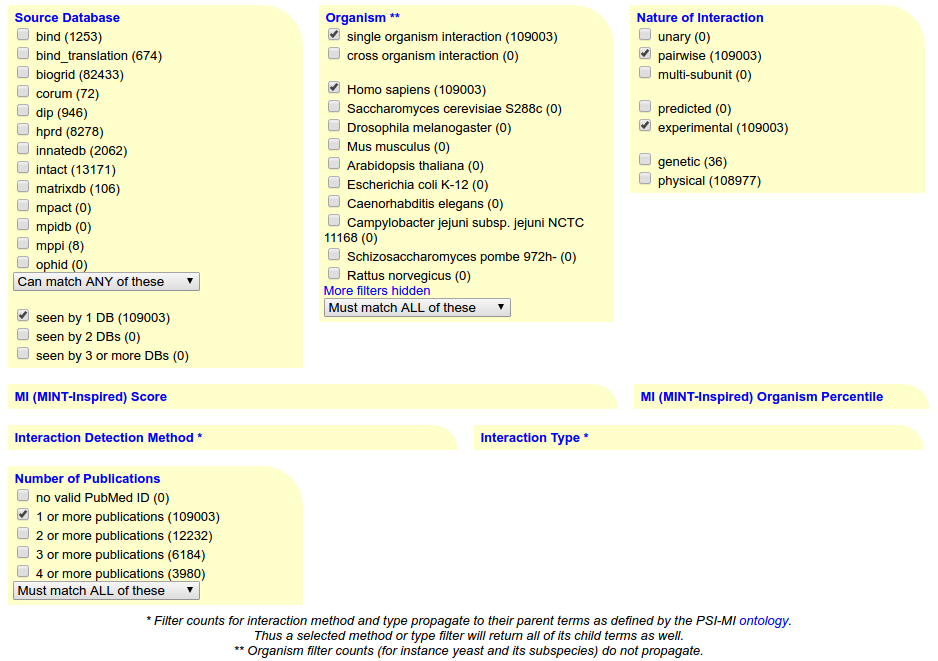
\includegraphics[width=15cm]{mitab_lite_109276}
    \caption{iRefWeb network query}
    \label{fig:irefweb}
\end{figure}

\subsubsection{iRefWeb}
It was downloaded in the MITAB-MINI format. A python script cleaned up the file,
leaving only the aliases for the source and target proteins. This result was
matched up against genes from HGNC. The HGNC data represents genes, and their
protein product. This way, the network would consist of genes instead of
proteins. This conversion was done in order to compare the end results from
ranking the clusters with genes that has connections to prostate cancer.
A criteria for the interactions retrieved from iRefWeb when converted from
proteins to genes was that both the source and target protein had to have
a match in the HGNC data, to not create any combinations of gene to protein or
protein to gene interactions. Duplicate interactions was not taken care of and
they did not occur in the network file either.

\subsubsection{COSMIC}
A network with only prostate cancer related genes from
COSMIC\cite{cosmic-download} was constructed with interaction information from
the iRefWeb network. This network was much smaller in terms of both nodes and
edges (interactions). The COSMIC network was created and ranked to see how
ranking a network with only cancer relevant genes would result in when data from
jensen was used to compare it to a much larger and generalized network.
Filtering the genes from COSMIC was done the same way as filtering the scores
for the genes; using only the COSMIC genes that contained genes from both ends,
source and target gene, of an interaction in the network.

\subsection{Score creation}
The golden standard for scoring that I used was created by data from
DisGeNET\cite{disgenet} and \gls{dragon}\cite{dragon}. 

DisGeNET is a database that is one of todays largest repositories of information
between diseases and genes.  It integrates expert-curated data with text mined
data. DisGeNET provides a score for genes related to a specific disease, in this
case prostate cancer.  This score is based on "the supporting evidence to
prioritize gene-disease associations"\cite{disgenet}. It also has a Cytoscape
plugin, but like iRefScape, it is outdated and can not be used together with
Cytoscape version 3.4.0. DisGeNET was chosen because of its comprehensive
collection of prostate cancer gene scores that was used as prior scores in both
\gls{prwp} and \gls{maa}.

\gls{dragon} is a knowledgebase of genes that is been experimentally verified as
an implicator in prostate cancer. It offers a bigger variety of information on
prostate cancer in general, as opposed to DisGeNET, but it does not have scores.
Therefore, to be used in the \gls{golden}, the genes from \gls{dragon} had to
receive a constructed score comparable to the scores from DisGeNET.

The DisGeNET data came with decimal scores from 0 to 1 and contained data about
several diseases, not only prostate cancer, and multiple instances of the same
gene could have multiple scores for different types of prostate cancer. The
duplication of gene entries with scores related to prostate cancer resulted in
a solution where the average of all of the prostate cancer scores created
a single score for a single gene. However, the data from \gls{dragon} did not
have any scores and was just a list with genes relevant to prostate cancer.  To
combine the two lists, the \gls{dragon} scores had to be converted to match the
DisGeNET scores. The method for converting the scores was to let the DisGeNET
scores be left as they were and try to add scores to the genes from the
\gls{dragon} data list. An average was created from the maximum and minimum
value from the DisGeNET scores. Then some sort of "sane" max value was created
by adding the average to a quarter of the value of the average value subtracted
from the maximum value.  This created a final value between the average and
maximum value that all of the \gls{dragon} genes received. The \gls{dragon}
genes receives on average a higher score than the DisGeNET genes because of the
way the lists are constructed. \gls{dragon} has no score, therefore they
signalize a proof of relevance to prostate cancer, while DisGeNET has a score
for how relevant the gene may be.

Finally, this golden standard of scores was filtered by removing any genes that
did not occur in the network. Because of the cross-validation performed after
the ranking of the clusters, the scores could not contain any genes not in the
network in order to not remove genes from the files with scores that would not
occur in the network. This would have resulted in a cross-validation where
a 100\% match never could happen.

\subsection{Creating scores for cross-validation}
A form of cross-validation was performed to assess how the ranking algorithms
performed alone and compared to each other. Creating the cross-validation scored
data sets required information about the clusters. Running MCL clustering on the
network and then export the node table in Cytoscape created the cluster basis
needed. From these clusters, it was possible to identify which clusters
contained scores that could be removed during cross-validation. A random 10\% of
the genes used for scoring was removed. Though, the amount of genes removed was
not totally random. There was set a rule that every cluster that contained genes
with a score from the golden standard, had to end up with keeping atleast 1 of
those genes. So in a cluster of 4, where 2 of them were scored in the golden
standard, that cluster could only lose 1 of those scored genes when the 10\% was
removed. Had this rule not been applied to the cross-validation, there would not
be a guarantee that 100\% of the removed genes would be found as candidate
genes. For \gls{maa} ranking, it would be impossible, and for \gls{pr}WP it
would be possible, but much less likely to find them. This is due to the simple
fact that clusters that go from having weighted nodes (genes), to having no
weighted genes, should not be ranked very high. The point of having weights is
to rely on prior information about cancer relation in genes and find cancer
candidate gene clusters by applying reason for "guilt-by-association" to the
genes that are not weighted.

\section{After running Ranklust}
\subsection{Exporting the data}
The data from performing Ranklust on the networks was exported as node tables
through Cytoscape. These tables contains information about each node, but not
any information about the edges. The scores added to the networks did not
involve any edge information, and for both of the algorithms used, \gls{maa} and
\gls{prwp}, the calculated scores are stored in the cluster, so there was no use
at this point to use the information in the edge table to find the cancer
candidate genes.

\subsection{Cleaning the data}
Cleaning the data was done in Python with its table manipulation library,
Pandas\cite{pandas}. The cleaning removed unnecessary data from the node table
files from exported from Cytoscape. The data still represents the same before
and after the cleaning, the difference is that the cleaned version is has tab
separated data, for better visual interpretation and it has less columns.

\textbf{Before cleaning:}
\begin{Verbatim}[fontsize=\scriptsize]
"SUID","__mclCluster","name","PRWP","PRWP_single","score","selected","shared name"
"72","25","FAM160B1","0.04478373407949736","7.818032875772688E-4",,"false","FAM160B1"
"73","6","APOPT1","0.04119274479140687","9.848244844960219E-4",,"false","APOPT1"
"74","6","FAM84A","0.04119274479140687","9.848244844960219E-4",,"false","FAM84A"
\end{Verbatim}

\textbf{After cleaning:}
\begin{Verbatim}[fontsize=\scriptsize]
__mclCluster	name	PRWP	score	PRWP_single
1136.0	CDC25C	1.0	0.272714418721	0.225926983193
1136.0	LZTS1	1.0	0.122995792115	0.197642927074
690.0	CREB3L4	0.918902810704	0.272714418721	0.189744545774
690.0	SCX	0.918902810704	0.0	0.102170140032
\end{Verbatim}

\begin{itemize}
    \item \_\_mclCluster
        \begin{itemize}
            \item Which cluster the gene/node in this row belongs to
        \end{itemize}
    \item name
        \begin{itemize}
            \item The HGNC representation of this gene/node
        \end{itemize}
    \item PRWP 
        \begin{itemize}
            \item The score of the cluster to this gene/node belongs to
        \end{itemize}
    \item score 
        \begin{itemize}
            \item The prior score assigned to this gene/node
        \end{itemize}
    \item PRWP\_single
        \begin{itemize}
            \item The PageRank score assigned to this gene/node (not a column in \gls{maa})
        \end{itemize}
\end{itemize}

\subsection{Recreate the clusters}
The cleaned data was then aggregated into clusters represented in text format.

\textbf{Combined clusters:}
\begin{Verbatim}[fontsize=\scriptsize]
clusters	score	genes
1136	1.0	LZTS1:0.122995792115,CDC25C:0.272714418721
690	0.918902810704	SOX9:0.272714418721,SCX:0.0,CREB3L4:0.272714418721
1004	0.758524309337	MMP14:0.272714418721,MMP13:0.12
\end{Verbatim}

Here, the \textit{clusters}-column are the unique identifier, and not the
\textit{HGNC} identifier or the \textit{SUID}from the previous data. The score
column does not represent the same data as before, but rather the same as the
PRWP column displayed in the cleaning examples, the total score of the cluster.
The genes column is double separated. The column itself is tab separated from
the other columns, the genes in it is separated with commas and the prior scores
belonging to each gene is delimited by a colon, not the \gls{prwp}/\gls{maa} or
any other algorithmic related score. This column contains all of the genes in
the cluster and aids in distinguishing the already proven biomarkers for cancer,
and the candidates.

\subsection{Cross-validation comparison}
Both \gls{prwp} and \gls{maa} had 10 cross-validated results each. Each
individual result from both of the algorithms was compared with the \gls{golden}
result created by each of the algorithms. This procedure was done to identify
the cancer biomarkers that existed in the \gls{golden} but ended up being
candidate cancer biomarkers in the cross-validation.

\subsection{Comparing with test data}
Matching the cluster ranks against test data is the last step in terms of
creating results that could reveal candidate network biomarkers for prostate
cancer. The procedure for matching cluster ranks with test data will consist of
inserting the test data genes with the cluster ranks. The test data genes will
be a single column list which contains unique genes proven to be prostate cancer
biomarkers. Creating a table with an overview of the test genes that match
the genes inside the ranked clusters, and whether the \gls{golden} classified
these ranked genes as prostate cancer genes or prostate cancer candidate genes,
is the final goal of this thesis. Traversing the ranked clusters and ascertain
which genes from the test data is inside which clusters and if they are
candidate biomarkers or already existing ones will end up producing the final
table used to represent the core result in this thesis. From creating and
scoring a network, cluster it, ranking it, assert its suitability to rank
clusters and present a final list of network candidate biomarkers for prostate
cancer.

The test data will come from three different sources. Manually expert curated
\gls{movember} from the Movember Prostate Cancer Project, prostate cancer genes
from experiments recorded in COSMIC\cite{cosmic-download}, and proven lethal
prostate cancer genes from an experiment that tried to reduce the amount of
over-treatment of prostate cancer based on screening from
PSA\cite{psa-overtreatment}. The three data sets will be mentioned as "movember"
for first set, "COSMIC" for the second, and "Lethal prostate cancer", or some
other context where "lethal" and "prostate" is mentioned together, for the
third.

All of this data can be found in the GitHub repository containing all of the raw
data and formatting scripts used in this assignment.

\textbf{Movember Prostate Cancer Project:}
\url{https://github.com/henninglh/data/blob/master/scoring/movember_corrected.txt}

\textbf{COSMIC:}
\url{https://github.com/henninglh/data/blob/master/scoring/cosmic_test.txt}

\textbf{Lethal prostate cancer:}
\url{https://github.com/henninglh/data/blob/master/scoring/lethal_cancer.txt}

\section{Plot creation}
The plots was created with an online tool named Plotly\cite{plotly}. Throughout
the whole process of creating plots, the X-axis represented the cluster ranks,
ordered from best to worst scored cluster, left to right, with ascending values
representing the ranks. The Y-axis represented in all cases an average. This
average was always calculated by dividing the sum of a specific value for each
gene, by the total number of genes in the cluster.

\section{Location of source code, data and scripts used in this assignment}
\begin{Verbatim}[fontsize=\scriptsize]
https://github.com/henninglh/ranklust-app
https://github.com/henninglh/data
https://github.com/henninglh/CyNeo4J
\end{Verbatim}

The first entry points to the source code of Ranklust. It contains the whole
clusterMaker2 source code combined with the Ranklust contribution, and can be
downloaded and compiled with the Java build tool Maven \cite{maven}.

The second entry is where all the data, that has been used at any point in the course
of this assignment, resides. It contains both the raw data and scripts to create
the data that was used to create the network, prior scores, benchmarks and test
data. Note: there exists scripts in this repository that was used at some point,
but their results did not make it into the thesis.

The third and last entry is where the changes to the CyNeo4j\cite{cyneo4j} app
for Cytoscape resides. It is complete with the changes mentioned in the future
work section of the Conclusion chapter. The changes enables the user to
connect to Neo4j servers that require authentication.
